
\section{Kubični interpolacijski splajn}

Kako bi se izbjegao navedeni problem s tranzicijom između segmenata, poželjno je konstruirati splajn višeg reda.
\textbf{Kvadratni splajn} može imati skokove prve derivacije u točkama mreže čvorova pa se on ne primjenjuje toliko često.
\textbf{Kubični splajn} se iznimno često koristi u praksi te nema nedostatke koje imaju linearni i kvadratni splajn.

Kada imamo zadane diskretne vrijednosti funkcije:

\begin{equation*}
y_i=f(x_i),\qquad i\in[0,n]
\end{equation*}

i čvorove zadane tako da vrijedi:

$$
a\leq x_0 < x_1 < \dots < x_n \leq b
$$

Kubični splajn je funkcija $s(x)\in\mathcal{C}^2(\langle x_0,x_n\rangle)$ koja je:

\begin{itemize}
    \item na svakom podintervalu $[x_i, x_{i+1}\rangle, i\in[0,n\rangle$ polinom najviše trećeg stupnja,
    \item u čvorovima interpolacije zadovoljava uvjete interpolacije te
    \item ima neprekidnu drugu derivaciju
\end{itemize}

Na svakom podintervalu koriste se polinomi:

\begin{equation*}
\phi[x_i,x_{i+1}] = p_i(x),\qquad i\in[0,n],\qquad p_i(x)\in\mathcal{P}_3
\end{equation*}

Kubični polinom $p_i(x)$ ima četiri koeficijenta, i može se zapisati u obliku:

$$
p_i(x)=a_0+a_1(x-x_i)+a_2(x-x_i)^2+a_3(x-x_i)^3
$$

\begin{conditionbox}[određivanje koeficijenata kubičnog splajna]
    \begin{align}
        p_0(x_0) =& y_0\nonumber\\
        \label{cs_continuation}
        p_{i-1}(x_i) = p_i(x_i) =& y_i,\qquad i\in[1,n-1]\\
        p_{n-1}(x_n) =& y_n\nonumber\\\nonumber\\
        \label{cs_continuation_fd}
        p'_{i}(x_{i+1}) = p'_{i+1}(x_{i+1}) =& y_i,\qquad i\in[0,n-2]\\
        \label{cs_continuation_sd}
        p''_{i}(x_{i+1}) = p''_{i+1}(x_{i+1}) =& y_i,\qquad i\in[0,n-2]\\\nonumber\\
        s_0=&f'(x_0)\nonumber\\
        \label{cs_slope}
        s_n=&f'(x_n)
    \end{align}

    \begin{itemize}
        \item Uvjet \ref{cs_continuation} osigurava neprekidnost interpolacije i daje $2n$ uvjeta.
        \item Uvjet \ref{cs_continuation_fd} osigurava neprekidnost prve derivacije na unutarnjim čvorovima interpolacije i daje $n-1$ uvjeta.
        \item Uvjet \ref{cs_continuation_sd} osigurava neprekidnost druge derivacije na unutarnjim čvorovima interpolacije i daje dodatnih $n-1$ uvjeta.
        \item Uvjet \ref{cs_slope} osigurava da je nagib interpolacije na rubovima segmenata jednak nagibu funkcije.
    \end{itemize}

    \ref{cs_slope} je jedan on različitih načina za zadati dodatne uvijete kako bi dobili jedinstvena rješenja kubičnog splajna, tj. moguće je postići jedinstvenost rješenja i na druge načine.
\end{conditionbox}

\newpage

Označimo derivacije u unutarnjim čvorovima

\begin{equation*}
s_i=\phi'(x_i),\qquad i\in[1,n-1]
\end{equation*}

Polinome $p_i(x)$ u ovom slučaju je najpraktičnije zapisati u Newtonovom obliku interpolacijskog polinoma

$$
\begin{array}{ccccc}
    x_i & f[x_i]\\
    & & s_i\\
    x_i&f[x_i] & & f[x_i,x_i,x_{i+1}]\\
    & & f[x_{i+1},x_i] & & f[x_i,x_i,x_{i+1},x_{i+1}]\\
    x_{i+1} & f[x_{i+1}] & & f[x_i,x_{i+1},x_{i+1}]\\
    & & s_i\\
    x_{i+1} & f[x_{i+1}]\\
\end{array}
$$

Gdje su $s_i=f'(x_i)=f[x_i,x_i]$, a $s_{i+1}=f'(x_{i+1})=f[x_{i+1},x_{i+1}]$.

Iz definicije Newtonovog polinoma slijedi:

\begin{gather*}
p_i(x) = f[x_i]+f[x_i,x_i](x-x_i) + f[x_i,x_i,x_{i+1}](x-x_i)^2\\
+f[x_i,x_i,x_{i+1},x_{i+1}](x-x_i)^2(x-x_{i+1})
\end{gather*}

Isti polinom se može zapisati i u bazi $(x-x_i)^k$ kao:

$$
p_i(x)=\sum_{k=0}^3a_k(x-x_i)^k
$$

\begin{align*}
a_0=&f[x_i]&\qquad a_1=&s_i\\\\
a_2=&\frac{f[x_i,x_{i+1}]-s_i}{h_i}&\qquad a_3=&\frac{s_{i+1}+s_i-2f[x_i,x_{i+1}]}{h_i^2}
\end{align*}

pri čemu je $h_i=x_{i+1}-x_i$.

Iz uvjeta \ref{cs_continuation}-\ref{cs_slope} proizlazi sustav:

$$
h_is_{i-1}+2(h_{i-1}+h_i)s_i+h_{i-1}s_{i+1}=3(h_if[x_{i-1},x_i]+h_{i-1}f[x_i,x_{i+1}]),\qquad i\in[1,n-1]
$$

Dobiveni sustav je sastavljen od $n-1$ jednadžbi s $n-1$ nepoznanica i strogo je dijagonalno dominantan po redcima pa zaključujemo da je determinanta sustava različita od 0, odnosno sustav ima jedinstveno rješenje $\{s_1,\dots,s_{n-1}\}$ čime je potpuno određen kubični splajn.

\subsection{Druga derivacija na rubu segmenta}

\begin{conditionbox}[druga derivacija ruba]
    Kao što je prethodno navedeno uvjet \ref{cs_slope} nije jedini način za postizanje jedinstvenih rješenja. Možemo ih postići i s:
    \begin{align}
        \phi''_0=&f''(x_0)\nonumber\\
        \label{cs_sd}
        \phi''_n=&f''(x_n)
    \end{align}
    Ovdje uvjet \ref{cs_sd} osigurava da je stopa promjene nagiba ("savijenost") na rubovima interpoliranih segmenata jednaka nagibu funkcije.
\end{conditionbox}

Uvjeti \ref{cs_continuation}, \ref{cs_continuation_fd}, \ref{cs_continuation_sd} i \ref{cs_sd} dovode do linearnog sustava od $n+1$ jednadžbe s $n+1$ nepoznanicom, odnosno

\begin{align*}
p''_1(x_0) =& f''(x_0)\\
h_is_{i-1}+2(h_{i-1}+h_i)s_i+h_{i-1}s_{i+1}=&3(h_if[x_{i-1},x_i]+h_{i-1}f[x_i,x_{i+1}])\\
p''_n(x_n) =& f''(x_n)
\end{align*}

Dobiveni sustav je dijagonalno dominantan po redcima pa postoji jedinstveno rješenje sustava $\{s_0,\dots,s_n\}$. Funkcija $\phi(x)$ je klase $\mathcal{C}^2[a,b]$. Ako funkcija $f(x)$ ima omeđenu četvrtu derivaciju, tada vrijedi

$$
f(x)=\phi(x) + \mathcal(O)(h^4),\qquad h\to0.
$$

\newpage

\begin{example}[uporaba kubičnog splajna]
    Primjenom kubičnog splajna odrediti $\phi(2.33)$ i $\phi(4.21)$ ako su zadani podaci:
    
    \center
    \begin{tabular}{r|c|c|c|c|c}
        $x$ & 1 & 2 & 3 & 4 & 5 \\
        \hline
        $f(x)$ & 1 & 0.5 & 0.333 & 0.25 & 0.2 \\
        \hline
        $f'(x)$ & -0.5 & -0.25 & -0.111 & -0.0625 & -0.04
    \end{tabular}
\end{example}

U zadanoj tablici vrijedi $s_i=f'(x_i)$. Traženi polinomi su oblika $p_i(x)=\sum_{k=0}^3a_k(x-x_i)^k$ pa prema sljedećem određujemo vrijednosti koeficijenata $a_0$, $a_1$, $a_2$, $a_3$ za svaki podsegment posebno.

Tablica podijeljenih razlika je

$$
\begin{array}{ccc}
1&1&\\
&&-0.5\\
2&0.5\\
&&-0.167\\
3&0.333\\
&&-0.083\\
4&0.25\\
&&0.05\\
5&0.2\\
\end{array}
$$

\begin{multicols}{2}
\begin{itemize}
\item Za $p_1(x)$ na intervalu $[1,2\rangle$ vrijedi:
    \begin{gather*}
    a_0=f(x_0)=1,\qquad a_1=s_0=-0.5,\\
    a_2=\frac{f[x_0,x_1]-s_0}{h}-h\cdot a_3=-0.25,\\
    a_3=\frac{s_0+s_1-2f[x_0,x_1]}{h^2}=0.25,\\
    p_1(x)=1-0.5(x-1)-0.25(x-1)^2\\+0.25(x-1)^3
    \end{gather*}
\item Za $p_2(x)$ na intervalu $[2,3\rangle$ vrijedi:
    \begin{gather*}
    a_0=f(x_1)=0.5,\qquad a_1=s_1=-0.25,\\
    a_2=\frac{f[x_1,x_2]-s_1}{h}-h\cdot a_3=0.11,\\
    a_3=\frac{s_1+s_2-2f[x_1,x_2]}{h^2}=-0.027,\\
    p_2(x)=0.5-0.25(x-2)-0.027(x-2)^2\\+0.11(x-2)^3
    \end{gather*}
\newcolumn
\item Za $p_3(x)$ na intervalu $[3,4\rangle$ vrijedi:
    \begin{gather*}
    a_0=f(x_2)=1,\qquad a_1=s_2=-0.111,\\
    a_2=\frac{f[x_2,x_3]-s_2}{h}-h\cdot a_3=0.0355,\\
    a_3=\frac{s_2+s_3-2f[x_2,x_3]}{h^2}=-0.0075,\\
    p_3(x)=0.333-0.111(x-3)+0.0355(x-3)^2\\-0.0075(x-3)^3
    \end{gather*}
\item Za $p_4(x)$ na intervalu $[4,5\rangle$ vrijedi:
    \begin{gather*}
    a_0=f(x_3)=0.25,\qquad a_1=s_3=-0.0625,\\
    a_2=\frac{f[x_3,x_4]-s_3}{h}-h\cdot a_3=0.0015,\\
    a_3=\frac{s_3+s_4-2f[x_3,x_4]}{h^2}=-0.0025,\\
    p_4(x)=0.25-0.0625(x-4)+0.0015(x-4)^2\\-0.0025(x-4)^3
    \end{gather*}
\end{itemize}
\end{multicols}

Konačno, $\Phi(2.33)=p_2(2.33)=0.4286$.

\begin{tikzpicture}
    \begin{axis}[
        domain=1:5,
        ymin=-1,ymax=1,
        ]
        \addplot[plotlinefound] expression[domain=1:2,samples=20]{1-0.5*(\x-1)-0.25*(\x-1)^2+0.25*(\x-1)^3} node[pos=0.5,anchor=south]{$p_1$};
        \addplot[plotlinefound,color=cGreen] expression[domain=2:3,samples=20]{0.5-0.25*(\x-2)-0.027*(\x-2)^2+0.11*(\x-2)^3} node[pos=0.5,anchor=south]{$p_2$};
        \addplot[plotlinefound,color=cYellow] expression[domain=3:4,samples=20]{0.333-0.111*(\x-3)+0.0355*(\x-3)^2-0.0075*(\x-3)^3} node[pos=0.5,anchor=south]{$p_3$};
        \addplot[plotlinefound,color=orange] expression[domain=4:5,samples=20]{0.25-0.0625*(\x-4)+0.0015*(\x-4)^2-0.0025*(\x-4)^3} node[pos=0.5,anchor=south]{$p_4$};
        \addplot[plotlinetarget] expression[domain=1:5,samples=100]{1/\x} node[pos=0.12,anchor=north]{$f(x)$};
        \addplot[plotinterpolated] coordinates {(1,1)};
        \addplot[plotinterpolated] coordinates {(2,0.5)};
        \addplot[plotinterpolated] coordinates {(3,0.333)};
        \addplot[plotinterpolated] coordinates {(4,0.25)};
        \addplot[plotinterpolated] coordinates {(5,0.2)};
    \end{axis}
\end{tikzpicture}

\newpage

\subsection{Određivanje kubičnog splajna u Pythonu}

\begin{example}
    Uporabom \codepkg{matplotlib} biblioteke, prikaži u Pythonu linearni splajn
    za podatke iz prethodnog primjera.
\end{example}

U sklopu \codepkg{scipy} biblioteke je u \codepkg{interpolate} modulu sadržana
\codefn{CubicSpline} funkcija koja računa kubičnu interpolaciju pomoću ulaznih
\verb|x| vrijednosti (prvi argument) i njima sukladnih \verb|y| vrijednosti
(drugi agrument), te kao rezultat daje formulu za interpolaciju.

\begin{multicols}{2}
    \input{../code/kub_spline.tex}

    \columnbreak

    \textbf{Rezultat prikaza}

    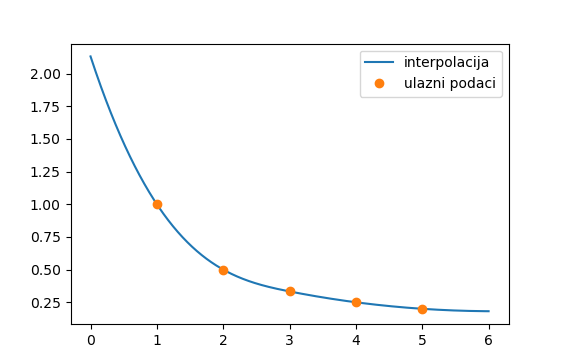
\includegraphics[width=\linewidth]{fig/kub_splajn.png}
\end{multicols}

Prethodno se koristila \codepkg{scipy.interpolate.}\codefn{interp1d} funkcija s argumentom \codenamedarg{kind}{\codestr{"cubic"}}.

\subsection{Greška kubičnog splajna}

Za kubični splajn ocjena greške je

\begin{align}
|f(x)-\phi(x)|\leq&\frac{\text{M}_4}{4!}\frac{h^4}{16}={1\over384}h^4\text{M}_4,\\
\text{M}_4=&\max_{x\in[a,b]}|f^{(IV)}(x)|,\\
h=&\max_{i\in[1,n]}h_i,\qquad h_i=x_{i+1}-x_i.
\end{align}

Drugim rjećima, ravnomjernim povećavanjem čvorova kubičnog splajna tako da $h\to0$, maksimalna greška te interpolacije se približava 0.
